\chapter{Physical Design}
\label{pd}
The physical design of the unit has been achieved by the usage of a script (see Appendix \ref{appendix12}). As for the synthesis, this script is in charge of preparing the environment and start the real script for the physical design.\\ This step is very well known as a computing intensive step, even more than the synthesis since the granularity of details is bigger than the one in the synthesis. Therefore, for boosting-up the performance the script automatically sets the usage of six threads instead of only one.\\\\
Nevertheless the variety in the design space, only a subset of them has been chosen for being placed on a die. In particular the unconstrained design, the minimum area and a 1\% more of the clock frequency (wrt to the non-constrained design clock's frequency) and only the 10\% more of the clock frequency designs. It is worth to mention that the physical design does not use the RTL description but it uses the gate-level netlist of the RTL, produced by the synthesis.\\
\section{Results}
In the following pages, results are presented as images of the design on the same die.\\
As first result of physical design, it is worth to present the ameba view. It distinguish between the control unit and the datapath of the DLX. As it can be seen from Figure \ref{fig:amebano} to Figure \ref{fig:ameba1minarea}, the area occupied by the control unit is always the same.\\\\
Moreover, from Figure \ref{fig:ameba} and Figure \ref{fig:place} it may seem that the pins are overlapping. However, this is not the case, it is only a matter of image resolution. Specifically, the pins on the top and right side (respectively for the IRAM and DRAM) are overlapped but on different level of the die. On the other hand, all the control signals from/to memories, clock and reset signals are on the bottom of the left corner.\\\\


\begin{figure}[!htbp]
  \centering
  \begin{subfigure}[b]{0.4\linewidth}
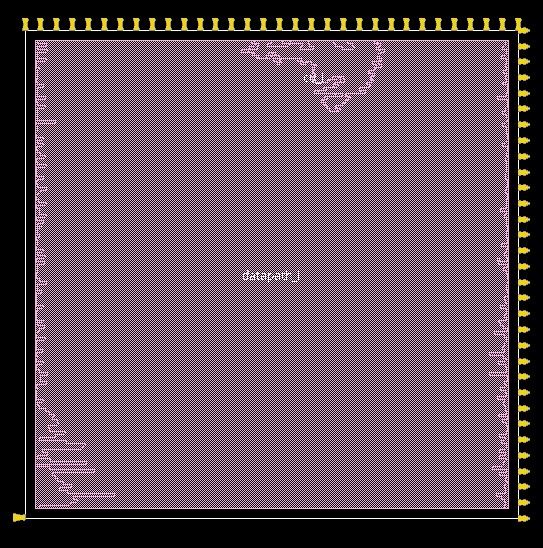
\includegraphics[width=\linewidth,scale=0.6,angle=0]{../project/physical_design/images_nopt/DLX_IR_SIZE32_PC_SIZE32_nopt_ameba_prerouting.jpg}
\caption{Unconstrained design}
\label{fig:amebano}
  \end{subfigure}
  \begin{subfigure}[b]{0.4\linewidth}
   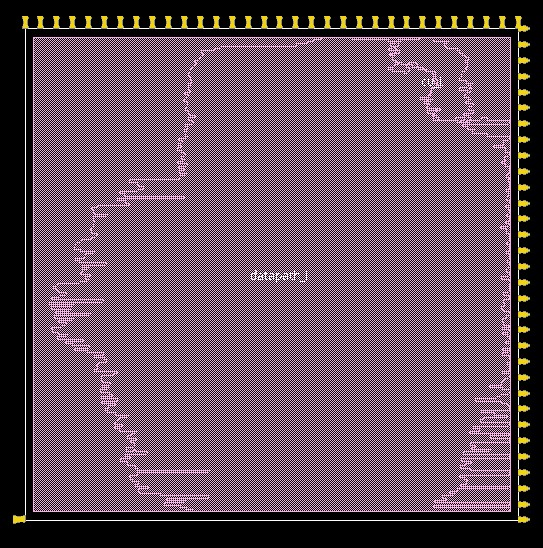
\includegraphics[width=\linewidth,scale=0.6,angle=0]{../project/physical_design/images_10/DLX_IR_SIZE32_PC_SIZE32_10_ameba_prerouting.jpg}
\caption{10\% more on clock frequency}
\label{fig:ameba10}
  \end{subfigure}
  
    \begin{subfigure}[b]{0.4\linewidth}
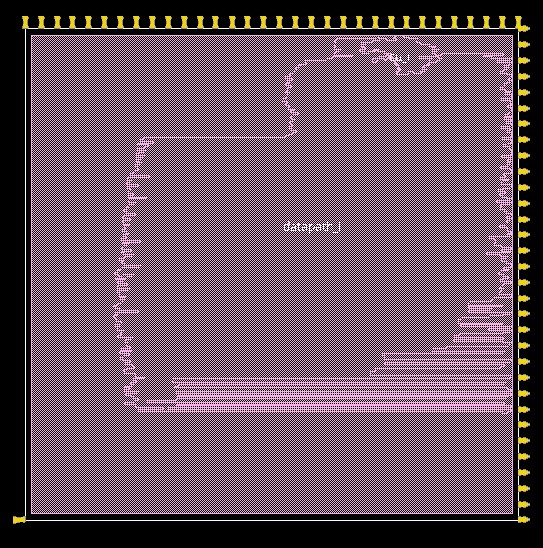
\includegraphics[width=1\linewidth,scale=0.6,angle=0]{../project/physical_design/images_1_minarea/DLX_IR_SIZE32_PC_SIZE32_1_minarea_ameba_prerouting.jpg}
\caption{1\% more on clock frequency and minimum area}
\label{fig:ameba1minarea}
  \end{subfigure}
\caption{Ameba view}
  \label{fig:ameba}
\end{figure}

An important aspect is how the datapath area is changing, having in mind the boundaries of datapath from Figures \ref{fig:ameba} and looking at Figures \ref{fig:place}. From A to C there is a consistent area reduction, the area is reducing by a factor of almost 2, this is mainly due to the area constraint and/or the relaxation on clock constraint. Comparing the Figure \ref{fig:placno} with the Figure \ref{fig:plac10}, even if there is a slight increase in the clock frequency, the synthesis strategies are different (it goes from a naive synthesis to a synthesis in which better optimization efforts are done in order to reduce design metrics). \\Therefore, even with a bigger clock frequency the final result is better than the non-constrained synthesis. The only difference with Figure \ref{fig:plac1minarea} is the constraint on finding the design with the minimum area and a lower increase in the clock frequency(only 1\%). The mix of those constrains has leaded to a further reduction in the area on the die.

\begin{figure}[!htbp]
  \centering
  \begin{subfigure}[b]{0.4\linewidth}
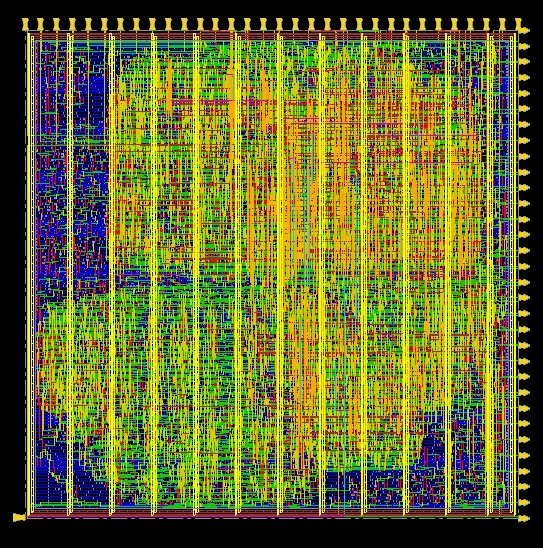
\includegraphics[width=\linewidth,scale=0.6,angle=0]{../project/physical_design/images_nopt/DLX_IR_SIZE32_PC_SIZE32_nopt_place_prerouting.jpg}
\caption{Unconstrained design}
\label{fig:placno}
  \end{subfigure}
  \begin{subfigure}[b]{0.4\linewidth}
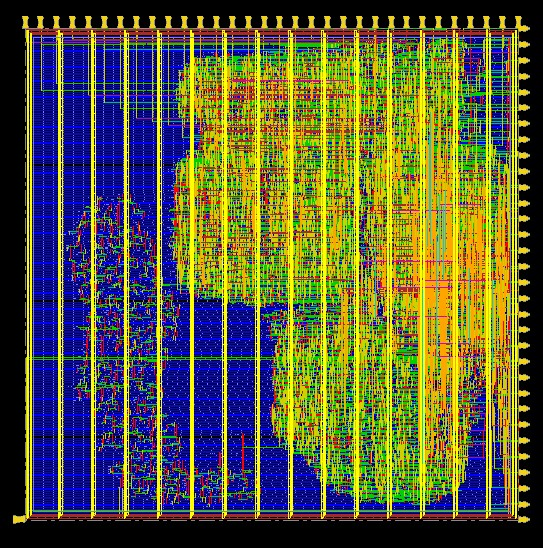
\includegraphics[width=\linewidth,scale=0.6,angle=0]{../project/physical_design/images_10/DLX_IR_SIZE32_PC_SIZE32_10_place_prerouting.jpg}
\caption{10\% more on clock frequency}
\label{fig:plac10}
  \end{subfigure}
  
    \begin{subfigure}[b]{0.4\linewidth}
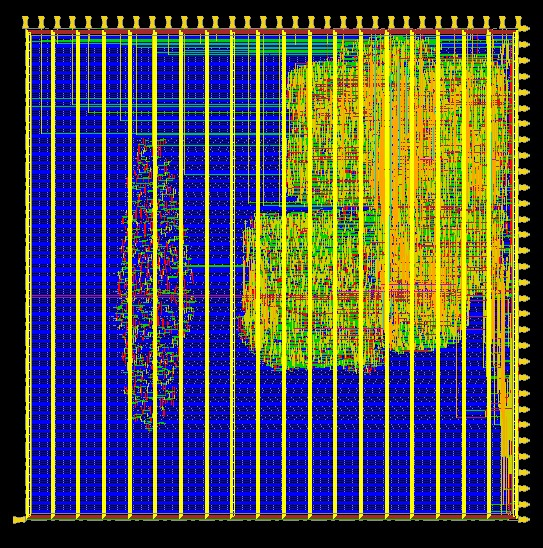
\includegraphics[width=1\linewidth,scale=0.6,angle=0]{../project/physical_design/images_1_minarea/DLX_IR_SIZE32_PC_SIZE32_1_minarea_place_prerouting.jpg}
\caption{1\% more on clock frequency and minumum area}
\label{fig:plac1minarea}
  \end{subfigure}
\caption{Placement view}
  \label{fig:place}
\end{figure}
